\documentclass[10pt,a4paper]{article}
\usepackage[utf8]{inputenc}
\usepackage[T1]{fontenc}
\usepackage[a4paper,top=1.5cm,bottom=1.5cm,left=1.5cm,right=1.5cm]{geometry}
\usepackage{amsmath}
\usepackage{amssymb}
\usepackage{tikz}
\usepackage{pgfplots}
\pgfplotsset{compat=1.18}
\pgfplotsset{
  grafik/.style={
    axis lines=middle,
    xlabel={$x$}, ylabel={$y$},
    width=7.5cm, height=6cm,
    grid=major, grid style={gray!25},
    tick label style={font=\scriptsize},
    every axis x label/.style={at={(ticklabel* cs:1)},anchor=west},
    every axis y label/.style={at={(ticklabel* cs:1)},anchor=south},
    title style={yshift=2ex},
  },
}
\usepackage[dvipsnames,svgnames]{xcolor}
\usepackage{booktabs}
\usepackage{tabularx}
\usepackage{array}
\usepackage[bookmarks=false]{hyperref}

\title{Rubrik Nilai Tugas Minggu 3 : Fungsi}
\author{Matematika untuk Sistem Informasi}
\date{}

\newenvironment{rubrik}{%
  \noindent
  \tabularx{\textwidth}{@{}>{\raggedright\arraybackslash}p{2.2cm}>{\raggedright\arraybackslash}X>{\centering\arraybackslash}p{1.1cm}>{\centering\arraybackslash}p{1.4cm}@{}}
  \toprule
  \textbf{Kriteria} & \textbf{Deskriptor} & \textbf{Maks} & \textbf{Skor} \\
  \midrule
}{%
  \bottomrule
  \endtabularx\par
}
\newcommand{\butir}[1]{\par\vspace{0.75em}\noindent\textbf{#1}\par\vspace{0.35em}}

\begin{document}
\maketitle

\noindent
Nama: \underline{\hspace{7.2cm}} \quad NIM: \underline{\hspace{4.2cm}}

\section*{Petunjuk penilai}
\begin{itemize}
  \item Tiap butir maksimum 100. Nilai tugas adalah rata-rata skor butir.
  \item Ketentuan skor:\par
  {\small
  \setlength{\tabcolsep}{4pt}%
  \begin{tabularx}{\linewidth}{@{}>{\raggedright\arraybackslash}p{2.1cm}>{\centering\arraybackslash}p{1.6cm}>{\raggedright\arraybackslash}X@{}}
  \toprule
  \textbf{Kriteria} & \textbf{Maks} & \textbf{Ketentuan} \\
  \midrule
  Langkah & 50 atau 60 & Jika langkah terbaca dan tidak seluruhnya salah, skor minimal 25. Skor di bawah 25 hanya bila langkah salah total, tidak dimengerti, atau tidak terbaca. \\
  Jawaban & 30 atau 40 & Harus ada dan benar. Skor hanya 0 atau nilai penuh. \\
  Penyajian & 20 & Harus ada dan benar. Skor hanya 0 atau nilai penuh. \\
  \bottomrule
  \end{tabularx}}
\end{itemize}

\butir{Butir 1(a). Domain dan range $f(x) = \sqrt{9 - x}$ (100 poin)}
\begin{rubrik}
Langkah &
Syarat radikan $9 - x \geq 0$ diselesaikan, dan range disimpulkan dari nilai akar yang nonnegatif. &
60 & \\
Jawaban &
$D_f = (-\infty, 9]$ dan $R_f = [0, \infty)$. &
40 & \\
\midrule
\multicolumn{2}{r}{\textbf{Jumlah}} & 100 & \\
\end{rubrik}

\butir{Butir 1(b). Domain dan range $f(x) = x^2 - 3x - 4$ (100 poin)}
\begin{rubrik}
Langkah &
Domain polinom dinyatakan, lalu range dari titik puncak parabola yang terbuka ke atas. &
60 & \\
Jawaban &
$D_f = \mathbb{R}$ dan $R_f = \bigl[-\frac{25}{4}, \infty\bigr)$. &
40 & \\
\midrule
\multicolumn{2}{r}{\textbf{Jumlah}} & 100 & \\
\end{rubrik}

\butir{Butir 2. Grafik fungsi (100 poin)}
\[
f(x) =
\begin{cases}
  x + 1, & x < -1 \\
  x^2, & -1 \le x < 2 \\
  2 - x, & x \ge 2
\end{cases}
\]
\begin{rubrik}
Langkah &
Nilai di ujung selang dihitung: lompatan di $x = -1$ (tinggi $0$ ke $1$) dan di $x = 2$ (tinggi $4$ ke $0$). &
50 & \\
Jawaban &
$D_f = \mathbb{R}$ dan $R_f = (-\infty, 4)$. &
30 & \\
Penyajian &
Grafik memuat garis, parabola, dan garis, dengan titik kosong dan titik penuh yang sesuai.\par\vspace{0.4em}
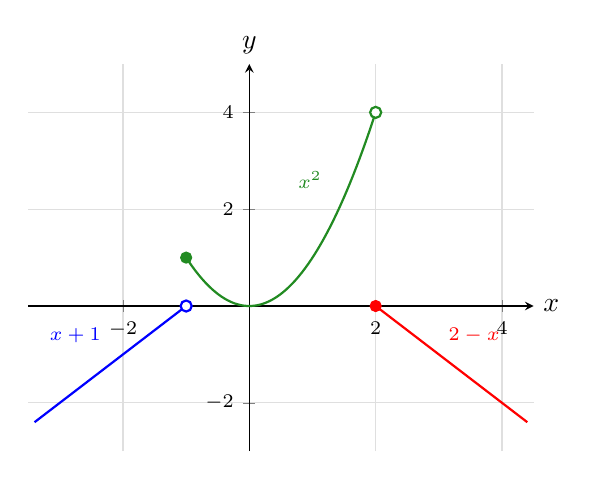
\begin{tikzpicture}
\begin{axis}[grafik, width=8cm, height=6.5cm, xmin=-3.5, xmax=4.5, ymin=-3, ymax=5]
  \addplot[domain=-3.4:-1, thick, blue] {x+1};
  \addplot[domain=-1:2, samples=60, thick, ForestGreen] {x^2};
  \addplot[domain=2:4.4, thick, Red] {2-x};
  \filldraw[blue, fill=white, thick] (axis cs:-1,0) circle (2pt);
  \filldraw[ForestGreen] (axis cs:-1,1) circle (2pt);
  \filldraw[ForestGreen, fill=white, thick] (axis cs:2,4) circle (2pt);
  \filldraw[Red] (axis cs:2,0) circle (2pt);
  \node[font=\scriptsize, blue, anchor=east] at (axis cs:-2.2,-0.6) {$x + 1$};
  \node[font=\scriptsize, ForestGreen, anchor=east] at (axis cs:1.3,2.6) {$x^2$};
  \node[font=\scriptsize, Red, anchor=west] at (axis cs:3,-0.6) {$2 - x$};
\end{axis}
\end{tikzpicture} &
20 & \\
\midrule
\multicolumn{2}{r}{\textbf{Jumlah}} & 100 & \\
\end{rubrik}

\butir{Butir 3. Grafik fungsi (100 poin)}
\[
f(x) =
\begin{cases}
  x, & x \le -1 \\
  x^2, & -1 < x < 2 \\
  3, & x \ge 2
\end{cases}
\]
\begin{rubrik}
Langkah &
Ujung selang diperiksa, termasuk titik kosong $(-1,1)$ dan $(2,4)$ serta nilai konstan $3$. &
50 & \\
Jawaban &
$D_f = \mathbb{R}$ dan $R_f = (-\infty, -1] \cup [0, 4)$. &
30 & \\
Penyajian &
Grafik memuat ketiga potongan dan membedakan titik penuh serta titik kosong.\par\vspace{0.4em}
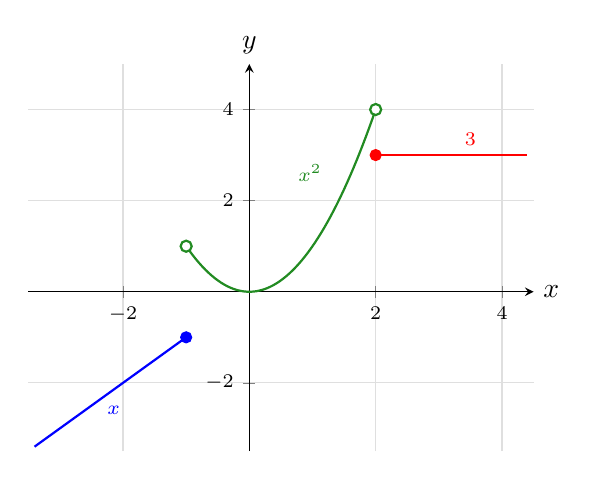
\begin{tikzpicture}
\begin{axis}[grafik, width=8cm, height=6.5cm, xmin=-3.5, xmax=4.5, ymin=-3.5, ymax=5]
  \addplot[domain=-3.4:-1, thick, blue] {x};
  \addplot[domain=-1:2, samples=60, thick, ForestGreen] {x^2};
  \addplot[domain=2:4.4, thick, Red] {3};
  \filldraw[blue] (axis cs:-1,-1) circle (2pt);
  \filldraw[ForestGreen, fill=white, thick] (axis cs:-1,1) circle (2pt);
  \filldraw[ForestGreen, fill=white, thick] (axis cs:2,4) circle (2pt);
  \filldraw[Red] (axis cs:2,3) circle (2pt);
  \node[font=\scriptsize, blue, anchor=west] at (axis cs:-2.4,-2.6) {$x$};
  \node[font=\scriptsize, ForestGreen, anchor=east] at (axis cs:1.3,2.6) {$x^2$};
  \node[font=\scriptsize, Red, anchor=south] at (axis cs:3.5,3) {$3$};
\end{axis}
\end{tikzpicture} &
20 & \\
\midrule
\multicolumn{2}{r}{\textbf{Jumlah}} & 100 & \\
\end{rubrik}

\butir{Butir 4. $f(x) = \sqrt{x}$, $g(x) = x^2$, komposisi $f \circ g$ (100 poin)}
\begin{rubrik}
Langkah &
Domain dan range $f$ serta $g$ dipakai untuk syarat $R_g \cap D_f \neq \emptyset$, lalu rumus, nilai, domain, dan range komposisi. &
60 & \\
Jawaban &
$f \circ g$ ada; $(f \circ g)(x) = |x|$, $(f \circ g)(5) = 5$, $D = \mathbb{R}$, $R = [0, \infty)$. &
40 & \\
\midrule
\multicolumn{2}{r}{\textbf{Jumlah}} & 100 & \\
\end{rubrik}

\butir{Butir 5. $f(x) = x^2$, $g(x) = x - 1$, komposisi $g \circ f$ (100 poin)}
\begin{rubrik}
Langkah &
Syarat irisan range dan domain diperiksa, lalu rumus, nilai di $x = 2$, domain, dan range. &
60 & \\
Jawaban &
$g \circ f$ ada; $(g \circ f)(x) = x^2 - 1$, $(g \circ f)(2) = 3$, $D = \mathbb{R}$, $R = [-1, \infty)$. &
40 & \\
\midrule
\multicolumn{2}{r}{\textbf{Jumlah}} & 100 & \\
\end{rubrik}

\butir{Butir 6. $f(x) = \sqrt{x-4}$, $g(x) = \sqrt{-1-x}$, komposisi $g \circ f$ (100 poin)}
\begin{rubrik}
Langkah &
$D_f = [4, \infty)$, $R_f = [0, \infty)$, $D_g = (-\infty, -1]$, lalu irisan $R_f \cap D_g$ diperiksa. &
60 & \\
Jawaban &
$g \circ f$ tidak ada karena irisannya kosong, sehingga rumus, domain, dan range komposisi tidak ditentukan. &
40 & \\
\midrule
\multicolumn{2}{r}{\textbf{Jumlah}} & 100 & \\
\end{rubrik}

\section*{Rekap skor}
\noindent
\begin{tabular}{@{}lr@{}}
\toprule
Butir & Skor \\
\midrule
1(a) & \\
1(b) & \\
2 & \\
3 & \\
4 & \\
5 & \\
6 & \\
\midrule
Rata-rata = jumlah skor / 7 (maksimum 100) & \\
\bottomrule
\end{tabular}

\end{document}
